\documentclass[../main.tex]{subfiles}
\begin{document}

% E' consentito agli studenti che ne facciano richiesta al proprio relatore, di formulare la tesi in lingua inglese e in ogni altra lingua straniera di uno stato dell’Unione Europea, purché il testo venga preceduto da un'ampia sintesi (dell'ordine di 10 pagine) dei contenuti in lingua italiana. All'atto della presentazione dei prescritti moduli in Segreteria studenti, il titolo della tesi dovrà essere definito sia in lingua italiana sia nella lingua straniera ed entrambe le formulazioni dovranno essere riportate sull'intestazione della tesi stessa.
\section{Sintesi italiana - Abstract}
Lo sviluppo software in ambito Automotive é un campo in continua espansione. Le linee di codice all'interno della centralina controllano tutti gli aspetti del veicolo, dalla temperatura nell'abitacolo, alla velocità su strada fino ai sistemi di guida autonoma ADAS. 
Le linee di codice presenti nei veicoli sono passate da quasi zero a qualche milione in un arco temporale di circa 50 anni. La crescita nella complessità ha richiesto una grande espansione nel campo dello sviluppo software per applicazioni autoveicolo. La complessità dietro i processi traspare nella prima parte della tesi, dove vengono analizzati i processi di sviluppo software all'interno del mondo Automotive, seguendo le metodologie usate presso \gls{BMW}.\\
Il focus si sposta poi sull'argomento principale della tesi, ovvero lo sviluppo di una pipeline dati per l'analisi di informazioni relative alle versioni di software per la centralina. Durante il ciclo di sviluppo software nella centralina una grande quantità di dati viene generata. Molto spesso questi dati vengono usati solamente dai dipartimenti responsabili dello sviluppo di una certa funzionalità e a volte, solamente dal singolo sviluppatore. Manca un sistema centralizzato che fornisca informazioni su tutto il processo.\\
Partendo da questa richiesta la tesi riporta il processo di sviluppo di un infrastruttura che possa attivamente salvare informazioni in un database e fornire un feedback agli sviluppatori tramite una visualizzazione grafica dei dati (Dashboard). Lo scopo del progetto é proprio questo, ovvero creare una Dashboard che possa fornire in tempo reale informazioni sullo stato di avanzamento dello sviluppo del software.\\
Il lavoro riportato nella tesi, parte con la creazione di un MVP, ovvero un primo prototipo atto a verificare la fattibilità della proposta e raccogliere un primo feedback sulla Dashboard. Dopodiché lo sviluppo continua con la creazione di una infrastruttura articolata che possa supportare il flusso id dati dal software, al database fino alla Dashboard. 

\section{Sintesi italiana - Introduzione}
Nel capitolo di introduzione viene trattato il tema del sistema automobile. Partendo da una semplificazione del modello automobile, riportato come semplice sistema ad anello chiuso la trattazione si sviluppa fino a definire la più complessa dicotomia elettronica meccanica nel veicolo, come riportato in Figura \ref{fig:schemaablocchi}.
\begin{figure}[ht]
        \begin{center}
  \begin{tikzpicture}[auto, node distance=3cm,>=latex', scale=0.7,transform shape]
            \node [input1, name=input] {};
            \node [sum1, right=of input] (sum) {};
            \node [sum, right=of sum] (sum_A) {};
            \node [block, right=of sum_A] (controller) {$Electronics$};
            \node [block, right=of controller] (mechanics) {$Mechanics$};
            \node [output1, right=of mechanics] (output) {};
            \draw [draw,->] (input) -- node {$User\; inputs$} (sum);
            \draw [->] (sum) -- node {} (sum_A);
            \draw [->] (sum_A) -- node {} (controller);
            \draw [->] (controller) -- node {} (mechanics);
            \draw [->] (mechanics) -- node [name=y] {$(speed,\; position..)$}(output);
            \draw [->] (mechanics) -- ++ (0,-2) -| node [pos=0.99] {$-$} (sum_A);
            \draw [->] (y) -- ++ (0,-4) -| node [pos=0.99] {$-$} (sum);
            % \node [container,fit=(controller) (mechanics) (sum_A)] (container) {};
            \end{tikzpicture}
        \end{center}
        \caption{Schema a blocchi di un'automobile}
        \label{fig:schemaablocchi}
    \end{figure}
La trattazione continua trattando il tema del software per centraline. In generale il software per \gls{ECU} può essere paragonato a software per sistemi embedded di tipo Real Time, ovvero dove la correttezza della risposta dipende non solo da una correttezza sul piano logico ma anche sul piano temporale. Con questo vengono di seguito introdotte le problematiche tipiche di sistemi real time, in modo da creare un'idea della complessità delle informazioni presenti nel software. 
Nella parte finale del capitolo viene poi introdotto il concetto di compilatore, il quale ha la funzione di ricevere come input il codice, sviluppato in Matlab che definisce il funzionamento della centralina e generare come output il codice compilato che potrà poi essere letto dall'organo centralina stesso.//
Il problema trattato nella tesi si lega a questo argomento. Infatti durante il processo di compilazione codice, il quale in \gls{BMW} è fatto da un compilatore sviluppato internamente, porta alla generazione di una grande mole di data riguardanti lo stato del processo. In generale differenti dipartimenti e differenti persone si occupano di singoli parti di questo processo. I dati non sono quindi solamente rilevanti in termine di mole ma sono anche divisi su differenti persone, rendendo complesso avere una visione d'insieme sullo stato del processo. A questo proposito l'obiettivo della tesi è quello di sviluppare una struttura che possa salvare i dati, processarli e fornirli a tutti gli utenti tramite una visualizzazione grafica. L'obiettivo di questo progetto è quello di migliorare il feedback per i singoli sviluppatori e fornire una visione d'insieme mancante. 
\section{Sintesi italiana - Agile e Scrum}
Il capitolo introduce e sviluppa concetti legati alle modalità di lavoro utilizzate nel campo dello sviluppo software. Inizialmente viene trattato il concetto di filosofia Agile, partendo da una breve introduzione storica fino alla prima teorizzazione, con i relativi punti salienti del Manifesto della filosofia Agile \cite{beck2001agile}. La trattazione dei modelli di lavoro Agile continua trattando alcune applicazioni reali della suddetta filosofia come lo Scrum (Figura \ref{fig:agilesrre}).\\
Scrum fornisce una struttura utile ad applicare modelli di lavoro Agile. La struttura si compone di vari parti, quali:
\begin{itemize}
    \item Scrum team, gruppo di persone con una gerarchia definita e all'interno del quale ogni persona ha un ruolo definito, legato allo Scrum.
    \item Eventi, il ciclo di sviluppo prodotto è basato su una serie di eventi, che insieme definiscono il cosiddetto Scrum Sprint.
    \item Regole, le quali uniscono e regolano non solo l'interazione tra ruoli ma definiscono anche ciò che accade nei singoli eventi e gli artefatti necessari per controllare l'intero processo.
\end{itemize}
Gli aspetti principali dello sviluppo prodotto secondo metodologie Scrum sono legati al continuo feedback all'interno del ciclo di lavoro, in modo da avere un costante miglioramento dell'output. Inoltre una ulteriore differenza con le metodologie di lavoro classiche si ritrova nella continua accettazione, durante tutto il ciclo di progettazione di nuove specifiche per il prodotto, aspetto che non si ritrova in metodologie classiche come i modelli di sviluppo a cascata.\\
Il capitolo tratta dunque in modo completo tutto ciò che riguarda la metodologia di lavoro Scrum, e la sua applicazione nel campo dello sviluppo software. In conclusione viene presentato un esempio di come un prodotto può essere sviluppato in modalità Scrum, facendo un paragone diretto con le metodologie classiche in modo tale da evidenziare le differenze e i punti di forza di entrambe.
\begin{figure}
    \centering
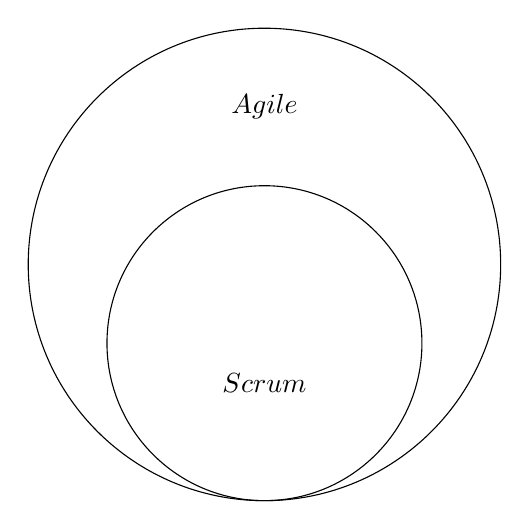
\begin{tikzpicture}
\draw[] (4.5,2) circle[radius = 3];
\node [at={(4.5,4)}] {$Agile$};
\draw [] (4.5,1) circle [radius =2];
\node [at = {(4.5,0.5)}] {$Scrum$};
\end{tikzpicture} 
    \caption{Relazione Agile - Scrum}
    \label{fig:agilesrre}
\end{figure}
\cleardoublepage
\end{document}